% Provenance (never printed): see sources/outline_sources.md (Year 1: vertical structure of
% the atmosphere, lapse rates, potential temperature and static stability; the layered
% ocean, the equation of state of seawater, T-S diagrams and water masses). Exercise and
% problem values in the Book 3 scratch calculator calc/ch26.py; figures from
% figdata/bachelor-1/atmosphere_profile.py (U.S. Standard Atmosphere 1976) and
% seawater_eos.py (EOS-80 and the UNESCO 44 algorithms; WOA23 columns, datasets
% bachelor-1-woa23-* and Book 2's grade-10-woa23-arctic-*).
% Physics owns the hydrostatic relation, the isothermal atmosphere and its scale height,
% the first law, Laplace's relation and Archimedes' thrust (recalled). Book 1 (g8) gave
% the layers and the environmental lapse rate of 6.5 K/km; Book 2 (g10) the dry adiabatic
% rate admitted, stable and unstable air, the mixed layer, thermocline, halocline and
% pycnocline: re-founded here with derivations. The moist adiabat is the Year 2 volume's.
\chapter{Structuur van de atmosfeer en de oceaan}\label{ch:b1:fluid-envelopes-structure}

Twee keer per dag wordt op weerstations over de hele wereld een ballon opgelaten die een radiosonde draagt, een klein instrument dat de druk, de temperatuur en de vochtigheid van de lucht terugzendt terwijl zij stijgt; zij klimt ongeveer \qty{300}{m} per minuut en kan \qty{35}{km} bereiken voordat de ballon barst. Ver op zee laat een onderzoeksschip een frame met instrumenten en watersleutels aan een kabel naar de diepzee zakken en meet de geleidbaarheid, de temperatuur en de diepte helemaal naar beneden. De twee profielen, één van de lucht en één van het water, zijn het ruwe materiaal van dit hoofdstuk. Beide omhulsels zijn gelaagd, en in beide wordt de laagvorming bepaald door de dichtheid: licht fluïdum boven zwaar fluïdum. Wat een laag licht of zwaar maakt, is minder vanzelfsprekend dan het lijkt. Lucht die kouder is dan de lucht eronder kan toch de lichtere zijn; water dat warmer is dan het water erboven kan toch het zwaardere zijn. Het hoofdstuk bouwt de twee hulpmiddelen die dit ordenen, de \omterm{def:b1:fluid-envelopes-structure:potential-temperature}{potentiële temperatuur} en de \omterm{def:b1:fluid-envelopes-structure:eos}{toestandsvergelijking van zeewater}.
% ledger: nws:radiosonde, nws:radiosonde-def, commons:ctd-rosette

\begin{omfigure}
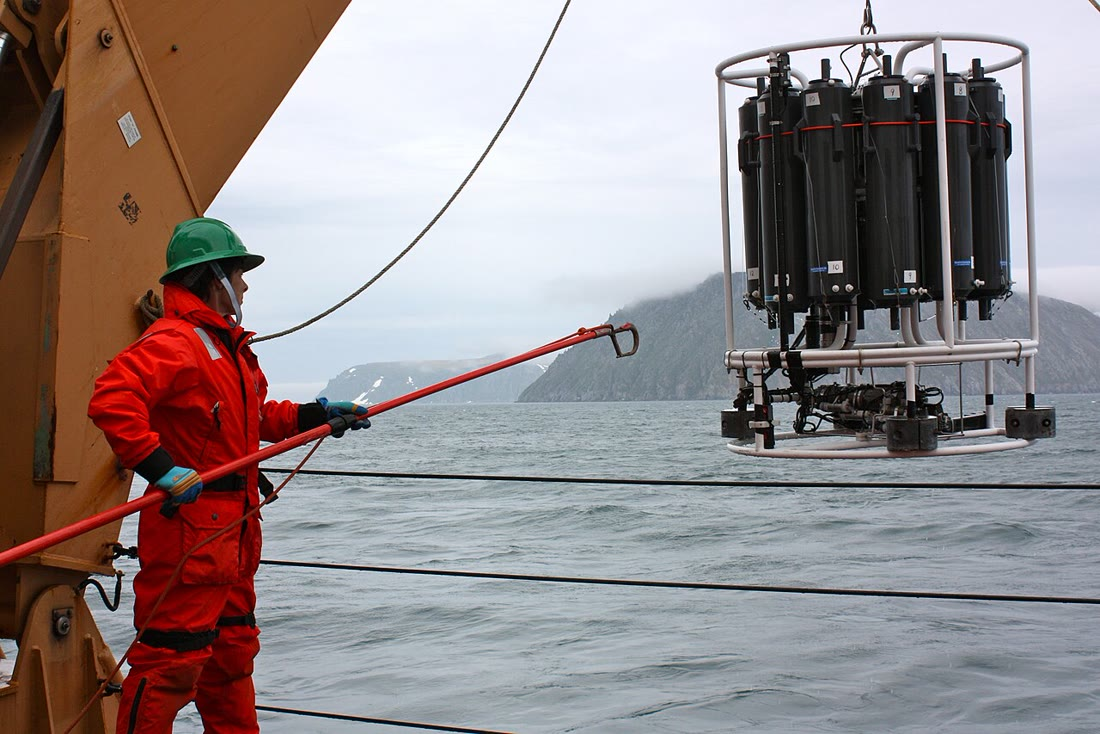
\includegraphics[width=0.62\linewidth]{images/book3/b1-ctd-rosette.jpg}

{\small Een CTD en een rozet worden in juni 2011 aan boord teruggehaald in de Beringstraat. De grijze flessen rond het frame worden op gekozen dieptes gesloten tijdens het opwaarts halen om het water te bemonsteren; de instrumenten onderaan het frame meten voortdurend de geleidbaarheid (waaruit het zoutgehalte wordt berekend), de temperatuur en de diepte (in feite de druk) terwijl het frame wordt neergelaten. (NASA Goddard Space Flight Center, publiek domein, via Wikimedia Commons.)}
\label{fig:b1:fluid-envelopes-structure:ctd}
\end{omfigure}
% ledger: commons:ctd-rosette, unesco44:atg-theta

\begin{recall}
De natuurkundeboeken geven de hydrostatische betrekking, $\mathrm dp/\mathrm dz =
-\rho g$, voor een fluïdum in rust; voor een ideaal gas van molaire massa $M$ geldt $p = \rho R
T/M$, en in een isotherme atmosfeer daalt de druk als $e^{-z/H}$ met de schaalhoogte $H = RT/(Mg)$. Zij formuleren de eerste hoofdwet voor een gesloten systeem en, voor een ideaal gas, de relatie van Laplace langs een omkeerbare adiabatische transformatie, $pV^{\gamma} = $ constant, met $\gamma = c_p/c_v$ en $c_p - c_v
= R/M$ per eenheid van massa. Een lichaam dat in een fluïdum wordt ondergedompeld, ontvangt een opwaartse stuwkracht gelijk aan het gewicht van het verplaatste fluïdum (Archimedes). Boek~1 noemde de lagen van de atmosfeer en de \omterm{def:b1:fluid-envelopes-structure:lapse-rate}{omgevingsgradiënt} van de \omterm{def:b1:fluid-envelopes-structure:standard-atmosphere}{standaardatmosfeer}, \qty{6.5}{\celsius} per kilometer in de troposfeer; Boek~2 aanvaardde de \omterm{def:b1:fluid-envelopes-structure:lapse-rate}{droogadiabatische gradiënt}, \qty{9.8}{\celsius} per kilometer, noemde lucht stabiel of labiel naargelang het lot van een pakketje dat omhoog wordt geduwd, en beschreef de \omterm{def:b1:fluid-envelopes-structure:ocean-layers}{gemengde laag}, de \omterm{def:b1:fluid-envelopes-structure:ocean-layers}{thermoklien}, de \omterm{def:b1:fluid-envelopes-structure:ocean-layers}{haloklien} en de \omterm{def:b1:fluid-envelopes-structure:ocean-layers}{pyklien} van de oceaan. Het zoutgehalte van zeewater is dicht bij \num{35} gram opgeloste zouten per kilogram.
% ledger: ussa76:layers, nws:dalr, nos:salinity
\end{recall}

\section{De verticale structuur van de atmosfeer}\label{sec:b1:fluid-envelopes-structure:atmosphere}

Geen enkele werkelijke sondering is gelijk aan de volgende. Om ze te vergelijken wordt bij conventie een referentieprofiel vastgelegd.

\begin{definition}[Standaardatmosfeer]\label{def:b1:fluid-envelopes-structure:standard-atmosphere}
Een \emph{standaardatmosfeer}\index{standaardatmosfeer} is een profiel van temperatuur, druk en dichtheid tegen de hoogte, bij conventie vastgelegd: droge lucht van constante molaire massa, een ideaal gas in hydrostatisch evenwicht, met gegeven waarden aan zeeniveau en een temperatuur die lineair met de hoogte varieert in opeenvolgende lagen. De standaardatmosfeer van 1976 neemt \qty{288.15}{K} en \qty{101325}{Pa} aan zeeniveau, $M_0 = \qty{28.9644}{kg.kmol^{-1}}$, $R^* = \qty{8314.32}{J.kmol^{-1}.K^{-1}}$ en $g_0 = \qty{9.80665}{m.s^{-2}}$.
\end{definition}
% ledger: ussa76:sea-level

Beneden \qty{47}{km} heeft de standaard van 1976 vier lagen (\cref{tab:b1:fluid-envelopes-structure:layers}). De laagste, de troposfeer, koelt af met \qty{6.5}{K} per kilometer; vanaf haar top, de tropopauze, blijft de temperatuur negen kilometer lang op \qty{216.65}{K}, en stijgt dan. De hoogten van de standaard zijn geopotentiële hoogten, de hoogten die een constante zwaartekracht $g_0$ dezelfde potentiële energie zou geven; beneden \qty{32}{km} verschillen zij minder dan \qty{0.6}{\percent} van geometrische hoogten (\qty{11}{km} van de standaard ligt op \qty{11.02}{km}).
% ledger: ussa76:layers, ussa76:sea-level

\begin{table}[ht]
\centering
\small
\renewcommand{\arraystretch}{1.2}
\begin{tabular}{|l|c|c|c|c|}
\hline
Laag & Basis (km) & $\mathrm dT/\mathrm dz$ (K/km) & $T$ aan de basis (K) & $p$ aan de basis (hPa) \\
\hline
1 (troposfeer) & 0 & $-6.5$ & 288.15 & 1013.25 \\
2 (stratosfeer) & 11 & 0.0 & 216.65 & 226.32 \\
3 (stratosfeer) & 20 & $+1.0$ & 216.65 & 54.75 \\
4 (stratosfeer) & 32 & $+2.8$ & 228.65 & 8.68 \\
\hline
\end{tabular}
\caption{De vier laagste lagen van de \omterm{def:b1:fluid-envelopes-structure:standard-atmosphere}{standaardatmosfeer} van 1976. De gradiënten en de waarden aan zeeniveau zijn vastleggende waarden; de temperaturen en drukken aan de basis worden daaruit berekend met \cref{prop:b1:fluid-envelopes-structure:layer-pressure}.}
\label{tab:b1:fluid-envelopes-structure:layers}
\end{table}
% ledger: ussa76:layers, ussa76:sea-level (bases computed in figdata/bachelor-1/atmosphere_profile.py)

In elke laag is de temperatuur een lineaire functie van de hoogte, zodat de hydrostatische betrekking in gesloten vorm kan worden geïntegreerd.

\begin{proposition}[Druk in een laag met constante gradiënt]\label{prop:b1:fluid-envelopes-structure:layer-pressure}
In een laag droge lucht waar $T = T_b - L\,(z - z_b)$ met een constante $L \neq 0$, is de druk
\[
  p = p_b \left(\frac{T}{T_b}\right)^{gM/(RL)},
\]
waarin $T_b$ en $p_b$ de waarden zijn aan de basis $z_b$. Wanneer $L = 0$ daalt de druk exponentieel met de schaalhoogte $H = RT_b/(Mg)$.
\end{proposition}

\begin{proof}
De hydrostatische betrekking en het ideale gas geven $\mathrm dp/p = -(gM/R)\,\mathrm
dz/T$. Aangezien $\mathrm dT = -L\,\mathrm dz$, is dit $\mathrm dp/p =
(gM/(RL))\,\mathrm dT/T$, wat integreert tot $\ln(p/p_b) = (gM/(RL))
\ln(T/T_b)$. Voor $L = 0$ is $T = T_b$ en $\ln(p/p_b) = -(z - z_b)/H$: de
isotherme atmosfeer van de natuurkundeboeken.
\end{proof}

In de troposfeer van de standaard is $gM/(RL) = 9.80665 \times 28.9644 /
(8314.32 \times 0.0065) = 5.256$, en op \qty{11}{km} is $T = 216.65$~K:
$p = \num{101325} \times (216.65/288.15)^{5.256} = \qty{22632}{Pa}$, iets
minder dan een kwart van de waarde aan zeeniveau. In de isotherme laag erboven is $H =
8314.32 \times 216.65/(28.9644 \times 9.80665) = \qty{6.34}{km}$, en negen
kilometer hoger is de druk met een verdere factor $e^{9/6.34} =
4.13$ gedaald, tot \qty{5475}{Pa}. Aangezien de druk op een niveau het gewicht is, per
oppervlakte-eenheid, van de lucht erboven, ligt de helft van de massa van de \omterm{def:b1:fluid-envelopes-structure:standard-atmosphere}{standaardatmosfeer} beneden
\qty{5.5}{km} en negen tiende beneden \qty{16}{km}.
% ledger: ussa76:sea-level, ussa76:layers (values computed in figdata/bachelor-1/atmosphere_profile.py)

\section{Verticale gradiënten en potentiële temperatuur}\label{sec:b1:fluid-envelopes-structure:lapse}

\begin{definition}[Omgevingsgradiënt en droogadiabatische gradiënt]\label{def:b1:fluid-envelopes-structure:lapse-rate}
De \emph{omgevingsgradiënt}\index{omgevingsgradiënt} is $\Gamma =
-\mathrm dT/\mathrm dz$, de snelheid waarmee de temperatuur van de lucht in rust met de hoogte daalt, zoals een sondering haar meet. De \emph{droogadiabatische
gradiënt}\index{droogadiabatische gradiënt} $\Gamma_d$ is de snelheid waarmee de temperatuur van een pakketje onverzadigde lucht daalt wanneer het pakketje wordt opgetild.
\end{definition}
% ledger: nws:dalr

Een gradiënt is positief wanneer de temperatuur met de hoogte daalt. De twee gradiënten zijn van verschillende aard: de eerste beschrijft de toestand van de atmosfeer op één moment; de tweede de transformatie van een stuk lucht dat beweegt.

\begin{definition}[Luchtpakketje]\label{def:b1:fluid-envelopes-structure:parcel}
Een \emph{luchtpakketje}\index{luchtpakketje} is een volume lucht dat in zijn beweging wordt gevolgd, klein genoeg om één temperatuur en één druk te hebben en de lucht eromheen niet te verstoren, groot genoeg om zijn identiteit te behouden: het wisselt geen massa uit en, tijdens een snelle verplaatsing, geen warmte met zijn omgeving, en zijn druk is op elk moment die van de omringende lucht.
\end{definition}

Het pakketje is een idealisatie, zoals het gesloten systeem van de thermodynamica: de onderstaande resultaten gelden voor werkelijke lucht voor zover een bewegend stuk ervan weinig warmte en weinig massa met zijn omgeving uitwisselt.

\begin{theorem}[De droogadiabatische gradiënt]\label{thm:b1:fluid-envelopes-structure:dry-adiabatic}
Een pakketje droge lucht, adiabatisch en omkeerbaar opgetild door lucht in rust van bijna dezelfde temperatuur, koelt af met de snelheid
\[
  \Gamma_d = \frac{g}{c_p},
\]
waarin $c_p$ de soortelijke warmte van lucht bij constante druk is. Met $c_p =
\qty{1004.7}{J.kg^{-1}.K^{-1}}$ is $\Gamma_d = \qty{9.76}{K.km^{-1}}$.
\end{theorem}

\begin{proof}
Voor een kilogram van het pakketje, met temperatuur $T_p$ en dichtheid $\rho_p$, is de eerste hoofdwet van een omkeerbare transformatie zonder warmte-uitwisseling, geschreven met de enthalpie, $c_p\,\mathrm dT_p - \mathrm dp/\rho_p = 0$. De druk van het pakketje is die van de lucht eromheen, die hydrostatisch is: $\mathrm dp = -\rho_e
g\,\mathrm dz$, met $\rho_e$ de dichtheid van de omringende lucht. Dus
\[
  \frac{\mathrm dT_p}{\mathrm dz} = -\frac{g}{c_p}\,\frac{\rho_e}{\rho_p}
  = -\frac{g}{c_p}\,\frac{T_p}{T_e},
\]
aangezien bij gelijke druk de dichtheden van twee ideale gassen van dezelfde molaire massa omgekeerd evenredig zijn met hun temperaturen. Wanneer het pakketje nagenoeg de temperatuur van zijn omgeving heeft, $T_p/T_e \approx 1$ en $-\mathrm dT_p/\mathrm dz
= g/c_p$. Voor droge lucht, een ideaal tweeatomig gas, $\gamma = 1.4$, dus $c_p =
\gamma/(\gamma - 1) \times R/M = 3.5 \times 8314.32/28.9644 =
\qty{1004.7}{J.kg^{-1}.K^{-1}}$, en $\Gamma_d = 9.80665/1004.7 =
\qty{0.00976}{K.m^{-1}}$.
\end{proof}
% ledger: nasa:grc-gamma, ussa76:sea-level, nws:dalr

Een pakketje \qty{10}{K} warmer dan zijn omgeving, nabij \qty{280}{K}, koelt af met
$\Gamma_d \times 290/280$, \qty{3.6}{\percent} sneller; de correctie wordt
in wat volgt verwaarloosd. De snelheid hangt niet af van de druk of de temperatuur van
het pakketje, en een pakketje dat zinkt warmt op met dezelfde snelheid, zoals Boek~2
lucht over een berg volgde.

Het integreren van dezelfde vergelijking zonder de hydrostatische stap geeft een grootheid die het pakketje met zich meedraagt.

\begin{proposition}[Potentiële temperatuur]\label{prop:b1:fluid-envelopes-structure:theta}
Langs een omkeerbare adiabatische transformatie van droge lucht,
\[
  \theta = T\left(\frac{p_0}{p}\right)^{\kappa},\qquad \kappa = \frac{R}{Mc_p} =
  \frac{\gamma - 1}{\gamma} = \frac{2}{7},
\]
blijft constant, wat de referentiedruk $p_0$ ook is.
\end{proposition}

\begin{proof}
Uit $c_p\,\mathrm dT = \mathrm dp/\rho$ en $\rho = pM/(RT)$ volgt $c_p\,\mathrm dT/T
= (R/M)\,\mathrm dp/p$, dus is $\ln T - \kappa \ln p$ constant, en dus ook $T
p^{-\kappa}$; vermenigvuldigen met de constante $p_0^{\kappa}$ geeft $\theta$. Dit is
de relatie van Laplace, geschreven met $T$ en $p$.
\end{proof}

\begin{definition}[Potentiële temperatuur]\label{def:b1:fluid-envelopes-structure:potential-temperature}
De \emph{potentiële temperatuur}\index{potentiële temperatuur} $\theta$ van een
pakketje droge lucht is de temperatuur die het zou hebben wanneer het adiabatisch naar
de referentiedruk $p_0 = \qty{1000}{hPa}$ wordt gebracht: $\theta = T\,(1000/p)^{2/7}$ met
$p$ in hectopascal en $T$ in kelvin.
\end{definition}
% ledger: nws:potential-temperature

De \omterm{def:b1:fluid-envelopes-structure:potential-temperature}{potentiële temperatuur} is een label dat een droog pakketje behoudt wanneer het stijgt of zinkt zonder warmte uit te wisselen, zoals het zoutgehalte van een waterpakketje dat doet. Verwarming door straling, door condensatie van water of door menging verandert het; de rest niet.

\begin{example}[De tropopauze van de standaardatmosfeer]\label{ex:b1:fluid-envelopes-structure:tropopause}
Aan het oppervlak van de standaard is $\theta = 288.15 \times (1000/1013.25)^{2/7} =
\qty{287.07}{K}$. Aan de tropopauze is $T = \qty{216.65}{K}$ en $p =
\qty{226.32}{hPa}$: $\theta = 216.65 \times (1000/226.32)^{2/7} = 216.65 \times
1.529 = \qty{331.2}{K}$. Lucht van de tropopauze die adiabatisch naar
\qty{1000}{hPa} wordt gebracht, zou \qty{331.2}{K} bereiken, \qty{44}{K} warmer dan oppervlaktelucht die naar dezelfde druk is gebracht. De temperatuur daalt met
\qty{71.5}{K} van de grond tot de tropopauze, en toch stijgt de \omterm{def:b1:fluid-envelopes-structure:potential-temperature}{potentiële temperatuur} met
\qty{44}{K}.
\end{example}
% ledger: ussa76:layers, nws:potential-temperature (values computed in figdata/bachelor-1/atmosphere_profile.py)

\section{Statische stabiliteit}\label{sec:b1:fluid-envelopes-structure:stability}

\begin{definition}[Statische stabiliteit; temperatuurinversie]\label{def:b1:fluid-envelopes-structure:stability}
De \emph{statische stabiliteit}\index{statische stabiliteit} van een laag in rust is haar reactie op een kleine verticale uitwijking van een pakketje. De laag heeft een \emph{stabiele gelaagdheid}\index{stabiele gelaagdheid} als het verplaatste pakketje terug wordt geduwd naar zijn niveau, een \emph{labiele
gelaagdheid}\index{labiele gelaagdheid} als het verder wordt weggeduwd, en een \emph{neutrale gelaagdheid}\index{neutrale gelaagdheid} als geen kracht erop werkt. Een \emph{temperatuurinversie}\index{temperatuurinversie} is een laag waarin de temperatuur met de hoogte stijgt.
\end{definition}
% ledger: nws:inversion

\begin{theorem}[Het criterium van statische stabiliteit]\label{thm:b1:fluid-envelopes-structure:stability}
Een laag droge lucht in rust, van temperatuur $T$ en \omterm{def:b1:fluid-envelopes-structure:lapse-rate}{omgevingsgradiënt} $\Gamma$, is stabiel als $\Gamma < \Gamma_d$, neutraal als $\Gamma = \Gamma_d$ en labiel als $\Gamma > \Gamma_d$; equivalent, zij is stabiel dan en slechts dan wanneer haar \omterm{def:b1:fluid-envelopes-structure:potential-temperature}{potentiële temperatuur} met de hoogte toeneemt. Een pakketje dat in een stabiele laag over een kleine $\delta z$ wordt verplaatst, oscilleert rond zijn niveau met de hoekfrequentie $N$, waarbij
\[
  N^2 = \frac{g}{T}\,(\Gamma_d - \Gamma) = \frac{g}{\theta}\,\frac{\mathrm d\theta}{\mathrm dz}.
\]
\end{theorem}

\begin{proof}
Een pakketje op de temperatuur $T$ van zijn niveau wordt over $\delta z$ opgetild. Het komt aan op $T - \Gamma_d\,\delta z$, terwijl de lucht eromheen op $T - \Gamma\,\delta z$ is. Per eenheid van massa voelt het pakketje zijn gewicht en de stuwkracht van Archimedes, een netto opwaartse versnelling $g\,(\rho_e - \rho_p)/\rho_p = g\,(T_p - T_e)/T_e$, de drukken zijn gelijk. In de eerste orde in $\delta z$ is dit
\[
  \frac{\mathrm d^2 \delta z}{\mathrm dt^2} = -\frac{g}{T}\,(\Gamma_d - \Gamma)\,\delta z = -N^2\,\delta z .
\]
Als $\Gamma < \Gamma_d$, is $N^2 > 0$ en oscilleert het pakketje met de hoekfrequentie $N$; als $\Gamma > \Gamma_d$ groeit de verplaatsing exponentieel; als $\Gamma = \Gamma_d$ werkt geen kracht. Voor de tweede vorm neemt men de logaritmische afgeleide van $\theta = T (p_0/p)^{\kappa}$ en gebruikt men de hydrostatische betrekking:
\[
  \frac{1}{\theta}\frac{\mathrm d\theta}{\mathrm dz} = \frac{1}{T}\frac{\mathrm dT}{\mathrm dz}
  - \frac{\kappa}{p}\frac{\mathrm dp}{\mathrm dz} = -\frac{\Gamma}{T} + \frac{\kappa\,\rho g}{p}
  = -\frac{\Gamma}{T} + \frac{\kappa g M}{RT} = \frac{\Gamma_d - \Gamma}{T},
\]
aangezien $\kappa M/R = 1/c_p$.
\end{proof}

De hoekfrequentie $N$ heet de drijffrequentie. In de troposfeer van de standaard, nabij de grond, is $N^2 = (9.80665/288.15) \times (9.761 -
6.5)\times10^{-3} = \qty{1.11e-4}{s^{-2}}$, $N = \qty{0.0105}{s^{-1}}$, en de
periode $2\pi/N$ van de oscillatie is ongeveer \qty{10}{min}. In de isotherme
lagere stratosfeer is $\Gamma = 0$: $N = \qty{0.0210}{s^{-1}}$, tweemaal zo groot, een
periode van vijf minuten. De stratosfeer is een deksel: zij weerstaat verticale beweging veel sterker dan de troposfeer eronder.
% ledger: ussa76:layers (values computed in figdata/bachelor-1/atmosphere_profile.py)

\begin{omfigure}
\begin{tikzpicture}
\begin{axis}[name=tz, omrecord, width=0.46\linewidth, height=7.2cm, xmin=160, xmax=300,
  ymin=0, ymax=32, xlabel={temperatuur (K)}, ylabel={hoogte (km)}, xtick={160,200,...,300},
  ytick={0,5,...,30}]
% figdata/bachelor-1/atmosphere_profile.py; ledger: ussa76:sea-level, ussa76:layers, nasa:grc-gamma
\addplot[omDef, line width=0.9pt] table[x=T_K, y=z_km] {figdata/out/bachelor-1-atmosphere_profile-profile.dat};
\addplot[omThm, dashed, line width=0.7pt] table[x=T_K, y=z_km] {figdata/out/bachelor-1-atmosphere_profile-adiabat.dat};
\addplot[only marks, mark=*, mark size=1.6pt, black] table[x=T_K, y=z_km] {figdata/out/bachelor-1-atmosphere_profile-tropo.dat};
\node[font=\scriptsize, text=omThm, anchor=west, align=left] at (axis cs:163,17.0) {droge adiabaat\\vanaf het oppervlak};
\node[font=\scriptsize, text=omDef, anchor=west] at (axis cs:252,6.4) {standaard};
\node[font=\scriptsize, anchor=east] at (axis cs:214.5,11.9) {tropopauze};
\end{axis}
\begin{axis}[at={(tz.east)}, anchor=west, xshift=1.3cm, omrecord, width=0.46\linewidth, height=7.2cm,
  xmin=250, xmax=900, ymin=0, ymax=32, xlabel={potentiële temperatuur (K)}, ylabel={hoogte (km)},
  xtick={300,500,700,900}, ytick={0,5,...,30}]
\addplot[omDef, line width=0.9pt] table[x=theta_K, y=z_km] {figdata/out/bachelor-1-atmosphere_profile-profile.dat};
\addplot[only marks, mark=*, mark size=1.6pt, black] table[x=theta_K, y=z_km] {figdata/out/bachelor-1-atmosphere_profile-tropo.dat};
\node[font=\scriptsize, anchor=west] at (axis cs:345,10.2) {\num{331} K};
\end{axis}
\end{tikzpicture}

{\small De \omterm{def:b1:fluid-envelopes-structure:standard-atmosphere}{standaardatmosfeer} van 1976 tot \qty{32}{km}. Links: temperatuur, met de droge adiabaat die een pakketje dat vanaf het oppervlak wordt opgetild zou volgen (gestreept). De standaard koelt langzamer af dan de adiabaat, en is dus overal stabiel. Rechts: \omterm{def:b1:fluid-envelopes-structure:potential-temperature}{potentiële temperatuur}, die overal met de hoogte stijgt, zacht in de troposfeer en steil boven de tropopauze (stip).}
\label{fig:b1:fluid-envelopes-structure:theta}
\end{omfigure}
% ledger: ussa76:sea-level, ussa76:layers, nasa:grc-gamma, nws:potential-temperature

Op een diagram van temperatuur tegen hoogte vergelijkt het criterium twee hellingen (figuur hieronder): het pakketje volgt de droge adiabaat door zijn startpunt, en de vraag is aan welke kant van de sondering het zich na een kleine verplaatsing bevindt.

\begin{omfigure}
\begin{tikzpicture}[x=0.55cm, y=0.55cm, >={Stealth[length=2mm]}]
\foreach \dx/\envtop/\verdict in {0/-0.8/{stabiele laag: het pakketje zakt terug}, 9/-3.8/{labiele laag: het pakketje stijgt door}} {
  \begin{scope}[xshift=\dx cm]
  \draw[->] (0,0) -- (7.2,0) node[below left, font=\scriptsize] {temperatuur};
  \draw[->] (0,0) -- (0,6.4) node[above right, font=\scriptsize] {hoogte};
  % sounding (environment): solid; dry adiabat through the starting point P: dashed
  \draw[omDef, line width=0.9pt] (5.0,0.6) -- (5.0+\envtop,5.4);
  \draw[omThm, dashed, line width=0.8pt] (5.0,0.6) -- (2.6,5.4);
  \fill (5.0,0.6) circle (2pt) node[right, font=\scriptsize] {$P$};
  \draw[densely dotted] (0,4.2) node[left, font=\scriptsize] {$z + \delta z$} -- (7,4.2);
  \fill[omThm] (3.2,4.2) circle (1.8pt);
  \fill[omDef] ({5.0+\envtop*3.6/4.8},4.2) circle (1.8pt);
  \node[font=\scriptsize, anchor=north] at (3.6,-0.5) {\verdict};
  \end{scope}
}
\end{tikzpicture}

{\small De pakketmethode. Volle blauwe lijn: de sondering; gestreepte rode lijn: de droge adiabaat door $P$. Een pakketje begint in $P$ op de temperatuur van de lucht eromheen en wordt langs de droge adiabaat opgetild naar $z + \delta z$ (rode stip); de sondering geeft de temperatuur van de lucht daar (blauwe stip). Links: de sondering koelt langzamer af dan de adiabaat; het pakketje komt kouder, dus dichter, aan dan zijn omgeving en zakt terug. Rechts: de sondering koelt sneller af dan de adiabaat; het pakketje komt warmer aan en blijft stijgen.}
\label{fig:b1:fluid-envelopes-structure:parcel}
\end{omfigure}

\begin{method}[De stabiliteit van een sondering lezen]\label{met:b1:fluid-envelopes-structure:sounding}
\begin{enumerate}
  \item Verdeel de sondering in lagen tussen niveaus waar de helling verandert.
  \item Bereken in elke laag $\Gamma = -(T_2 - T_1)/(z_2 - z_1)$, in kelvin per kilometer.
  \item Vergelijk met $\Gamma_d = \qty{9.8}{K/km}$: $\Gamma > \Gamma_d$ labiel, $\Gamma$ dicht bij $\Gamma_d$ neutraal, $\Gamma < \Gamma_d$ stabiel; een negatieve $\Gamma$ is een inversie, het meest stabiele geval.
  \item Waar drukken gegeven zijn in plaats van hoogten, bereken $\theta =
        T(1000/p)^{2/7}$ op elk niveau: $\theta$ die naar boven daalt markeert een labiele laag, constant een neutrale, stijgend een stabiele.
\end{enumerate}
\end{method}

Een labiele laag houdt niet lang stand: een verplaatsing erin groeit exponentieel, met de snelheid $\sqrt{-N^2}$, en de pakketten die zij vrijmaakt keren haar om, en mengen haar tot haar \omterm{def:b1:fluid-envelopes-structure:potential-temperature}{potentiële temperatuur} uniform is en haar gradiënt $\Gamma_d$ is. Een laag die van onderen wordt verwarmd, door warme grond of een warme zee, wordt naar labiliteit geduwd; een die van onderen wordt afgekoeld, naar stabiliteit. Een inversie bedekt alles wat eronder ligt: een pakketje dat van onderen opstijgt, komt kouder dan zijn omgeving te zitten zodra het erin binnengaat. Boven \qty{20}{km} is de hele stratosfeer van de standaard een inversie.

Dit alles veronderstelt droge lucht. Een opstijgend pakketje dat verzadigd raakt, komt vrij met latente warmte terwijl zijn water condenseert, en koelt langzamer af dan $\Gamma_d$; de verzadigde adiabaat en de voorwaardelijke labiliteit die zij meebrengt, zijn het onderwerp van Boek~4.
% ledger: nws:inversion, nws:dalr

\section{De gelaagde oceaan}\label{sec:b1:fluid-envelopes-structure:ocean}

De oceaan wisselt warmte en water met de atmosfeer alleen aan haar oppervlak, door verwarming en afkoeling, verdamping en regen. Haar verticale structuur heeft drie ingrediënten: temperatuur, zoutgehalte en dichtheid.

\begin{definition}[Gemengde laag, thermoklien, haloklien, pyklien]\label{def:b1:fluid-envelopes-structure:ocean-layers}
De \emph{gemengde laag}\index{gemengde laag} is de oppervlaktelaag van de oceaan waarvan temperatuur, zoutgehalte en dichtheid nagenoeg uniform zijn met de diepte; haar diepte wordt op een profiel afgelezen als de diepte waar de temperatuur voor het eerst met een gekozen drempel, vaak \qty{0.5}{\celsius}, van haar oppervlaktewaarde afwijkt. De \emph{thermoklien}\index{thermoklien}, de \emph{haloklien}\index{haloklien} en
de \emph{pyklien}\index{pyklien} zijn de lagen eronder waarin de temperatuur, het zoutgehalte en de dichtheid respectievelijk het snelst met de diepte veranderen.
\end{definition}

De druk in de oceaan wordt opgegeven in decibar, want één decibar, \qty{e4}{Pa}, is bijna de druk van één meter zeewater: op \qty{30}{\degree} \omterm{def:b1:spherical-astronomy:geographic}{breedtegraad} liggen \qty{1000}{dbar} op \qty{990.8}{m} en \qty{10000}{dbar} op \qty{9712.7}{m}.
% ledger: unesco:eos80-checks (DEPTH table computed in figdata/bachelor-1/seawater_eos.py)

Water is bijna onsamendrukbaar, maar niet helemaal, en een waterpakketje dat van diep water wordt opgetild zet uit en koelt een beetje af, zoals een \omterm{def:b1:fluid-envelopes-structure:parcel}{luchtpakketje} doet. De adiabatische gradiënt van zeewater is klein, ongeveer \qty{0.04}{\celsius} per \qty{1000}{dbar} aan het oppervlak bij \qty{0}{\celsius} en \qty{0.09}{\celsius} per \qty{1000}{dbar} op \qty{3000}{dbar}, tegen \num{9.8} per kilometer in lucht; maar over vijf kilometer telt het op tot enkele tienden van een graad, meer dan de verschillen tussen diepe wateren. Oceanografen vergelijken wateren daarom ook naar hun \emph{potentiële} temperatuur: de temperatuur die een pakketje zou hebben wanneer het adiabatisch, zonder verandering van zoutgehalte, naar het oppervlak wordt gebracht. Een water van \qty{2}{\celsius} op \qty{4000}{dbar} en zoutgehalte 35 heeft een \omterm{def:b1:fluid-envelopes-structure:potential-temperature}{potentiële temperatuur} van \qty{1.66}{\celsius}. In de diepste niveaus van de Zuid-Atlantische Oceaan op \qty{10.5}{\degree S} stijgt de gemeten temperatuur van \qty{0.730}{\celsius} op \qty{5400}{m} tot \qty{0.731}{\celsius} op \qty{5500}{m}, terwijl de \omterm{def:b1:fluid-envelopes-structure:potential-temperature}{potentiële temperatuur} daalt van \qty{0.261}{\celsius} tot \qty{0.250}{\celsius}: de opwarming is compressie, geen warmte.
% ledger: unesco44:atg-theta, data:b3-woa23 (values computed in figdata/bachelor-1/seawater_eos.py)

\begin{omfigure}
\begin{tikzpicture}
\begin{groupplot}[group style={group size=3 by 1, horizontal sep=0.55cm, yticklabels at=edge left},
  omrecord, omdepth, width=0.365\linewidth, height=7.4cm, ymin=0, ymax=2000,
  ytick={0,500,1000,1500,2000}, y tick label style={/pgf/number format/.cd, set thousands separator={}},
  every axis label/.append style={font=\small}]
\nextgroupplot[xmin=-2, xmax=28, xlabel={$\theta$ (\si{\celsius})}, ylabel={diepte (m)}, xtick={0,10,20}]
% figdata/bachelor-1/seawater_eos.py; WOA23 (datasets bachelor-1-woa23-*, grade-10-woa23-arctic-*); ledger: data:b3-woa23, data:b2-woa23, unesco44:atg-theta
\addplot[omThm, line width=0.8pt] table[x=theta, y=depth] {figdata/out/bachelor-1-seawater_eos-prof-sa10.dat};
\addplot[omProp, line width=0.8pt] table[x=theta, y=depth] {figdata/out/bachelor-1-seawater_eos-prof-sa30.dat};
\addplot[omDef, line width=0.8pt] table[x=theta, y=depth] {figdata/out/bachelor-1-seawater_eos-prof-arctic.dat};
\draw[omThm, line width=0.8pt] (axis cs:9,1250) -- (axis cs:13,1250) node[right, font=\scriptsize, text=black] {\qty{10.5}{\degree S}};
\draw[omProp, line width=0.8pt] (axis cs:9,1450) -- (axis cs:13,1450) node[right, font=\scriptsize, text=black] {\qty{30.5}{\degree S}};
\draw[omDef, line width=0.8pt] (axis cs:9,1650) -- (axis cs:13,1650) node[right, font=\scriptsize, text=black] {\qty{75.5}{\degree N}};
\nextgroupplot[xmin=28, xmax=37.5, xlabel={zoutgehalte}, xtick={28,31,34,37}]
\addplot[omThm, line width=0.8pt] table[x=s, y=depth] {figdata/out/bachelor-1-seawater_eos-prof-sa10.dat};
\addplot[omProp, line width=0.8pt] table[x=s, y=depth] {figdata/out/bachelor-1-seawater_eos-prof-sa30.dat};
\addplot[omDef, line width=0.8pt] table[x=s, y=depth] {figdata/out/bachelor-1-seawater_eos-prof-arctic.dat};
\nextgroupplot[xmin=22, xmax=28.5, xlabel={$\sigma_\theta$ (\si{kg.m^{-3}})}, xtick={22,24,26,28}]
\addplot[omThm, line width=0.8pt] table[x=sigma, y=depth] {figdata/out/bachelor-1-seawater_eos-prof-sa10.dat};
\addplot[omProp, line width=0.8pt] table[x=sigma, y=depth] {figdata/out/bachelor-1-seawater_eos-prof-sa30.dat};
\addplot[omDef, line width=0.8pt] table[x=sigma, y=depth] {figdata/out/bachelor-1-seawater_eos-prof-arctic.dat};
\end{groupplot}
\end{tikzpicture}

{\small \omterm{def:b1:fluid-envelopes-structure:potential-temperature}{Potentiële temperatuur}, zoutgehalte en potentiële \omterm{def:b1:fluid-envelopes-structure:eos}{dichtheidsanomalie} (\cref{def:b1:fluid-envelopes-structure:eos}) in de bovenste \qty{2000}{m}, in het jaargemiddelde, op drie plaatsen: de tropische Zuid-Atlantische Oceaan (\qty{10.5}{\degree S}, \qty{25.5}{\degree W}), de subtropische Zuid-Atlantische Oceaan (\qty{30.5}{\degree S}, \qty{25.5}{\degree W}) en het Canadabekken van de Noordelijke IJszee (\qty{75.5}{\degree N}, \qty{150.5}{\degree W}). Gegevens: World Ocean Atlas 2023.}
\label{fig:b1:fluid-envelopes-structure:profiles}
\end{omfigure}
% ledger: data:b3-woa23, data:b2-woa23, unesco:eos80, unesco44:atg-theta

De drie kolommen van de figuur hierboven tonen de drie soorten bovenste oceaan. In de tropen zit een warme \omterm{def:b1:fluid-envelopes-structure:ocean-layers}{gemengde laag} nabij \qty{26.5}{\celsius} op een scherpe \omterm{def:b1:fluid-envelopes-structure:ocean-layers}{thermoklien}: tussen \qty{100}{m} en \qty{200}{m} daalt de \omterm{def:b1:fluid-envelopes-structure:potential-temperature}{potentiële temperatuur} van \qty{24.0}{\celsius} tot \qty{14.4}{\celsius}, en de dichtheid volgt haar, zodat de \omterm{def:b1:fluid-envelopes-structure:ocean-layers}{thermoklien} ook de \omterm{def:b1:fluid-envelopes-structure:ocean-layers}{pyklien} is. Op \qty{30.5}{\degree S} is het oppervlak koeler, \qty{21.1}{\celsius}, en de daling geleidelijker, verspreid over de bovenste \qty{800}{m}. In beide is het zoutgehalte het hoogst nabij het oppervlak en neemt het naar beneden af; het werkt tegen de gelaagdheid in, die de temperatuur ruimschoots compenseert. De Arctische kolom is het tegenovergestelde geval. Haar oppervlaktewater, op \qty{-1.4}{\celsius}, is het koudste van de drie, en toch het lichtste, $\sigma_\theta = 22.5$, omdat haar zoutgehalte slechts \num{28.1} is; het zoutgehalte stijgt tot \num{34.5} op \qty{300}{m}. De \omterm{def:b1:fluid-envelopes-structure:ocean-layers}{haloklien} is hier de \omterm{def:b1:fluid-envelopes-structure:ocean-layers}{pyklien}. Daaronder ligt een laag warmer dan het water erboven, nabij \qty{0.7}{\celsius} op \qty{475}{m}: een \omterm{def:b1:fluid-envelopes-structure:stability}{temperatuurinversie} die volkomen stabiel is, neergedrukt door zijn zout.
% ledger: data:b3-woa23, data:b2-woa23 (values computed in figdata/bachelor-1/seawater_eos.py)

\section{Dichtheid van zeewater en T--S-diagrammen}\label{sec:b1:fluid-envelopes-structure:ts}

\begin{definition}[Toestandsvergelijking van zeewater; haline contractiecoëfficiënt; dichtheidsanomalie]\label{def:b1:fluid-envelopes-structure:eos}
De \emph{toestandsvergelijking van zeewater}\index{toestandsvergelijking van zeewater}
geeft zijn dichtheid $\rho(S, T, p)$ als functie van zoutgehalte, temperatuur en
druk. De \emph{haline contractiecoëfficiënt}\index{haline contractiecoëfficiënt}
is $\beta = (1/\rho)\,\partial\rho/\partial S$ bij constante temperatuur en druk. De \emph{dichtheidsanomalie}\index{dichtheidsanomalie}
$\sigma$ is een dichtheid min \qty{1000}{kg.m^{-3}}: $\sigma_t = \rho(S, T, 0) -
1000$ gebruikt de gemeten temperatuur bij nul zeedruk, en de potentiële dichtheidsanomalie $\sigma_\theta = \rho(S, \theta, 0) - 1000$ de
\omterm{def:b1:fluid-envelopes-structure:potential-temperature}{potentiële temperatuur}.
\end{definition}
% ledger: teos10:alpha-beta, teos10:sigma

De toestandsvergelijking is niet uit eerste beginselen afgeleid, maar aan laboratoriummetingen gepast. De internationale vergelijking van 1980 bij de druk van het oppervlak is een polynoom met vijftien coëfficiënten, $\rho = \rho_w(T) +
A(T)\,S + B(T)\,S^{3/2} + C\,S^2$, waarin $\rho_w$ de dichtheid van zuiver water is; zij geeft $\rho(35, \qty{0}{\celsius}) = \qty{1028.1063}{kg.m^{-3}}$. Een thermodynamische beschrijving van zeewater, TEOS-10, werd in 2009 aangenomen om haar als de officiële te vervangen; de vergelijking van 1980 wordt hier gebruikt omdat haar polynoom op een pagina past. Haar thermische uitzettingscoëfficiënt $\alpha = -(1/\rho)\,\partial\rho/\partial T$ is de coëfficiënt uit de natuurkundeboeken.
% ledger: unesco:eos80, teos10:alpha-beta, teos10:replaced

\begin{table}[ht]
\centering
\small
\renewcommand{\arraystretch}{1.2}
\begin{tabular}{|c|c|c|c|}
\hline
$T$ (\si{\celsius}) & $\rho(35, T, 0)$ (\si{kg.m^{-3}}) & $\alpha$ (\si{K^{-1}}) & $\beta$ \\
\hline
0 & 1028.106 & \num{0.53e-4} & \num{7.85e-4} \\
10 & 1026.952 & \num{1.67e-4} & \num{7.61e-4} \\
25 & 1023.343 & \num{2.97e-4} & \num{7.39e-4} \\
\hline
\end{tabular}
\caption{Dichtheid en uitzettingscoëfficiënten van zeewater met zoutgehalte 35 bij de oppervlaktedruk, uit de internationale toestandsvergelijking van 1980.}
\label{tab:b1:fluid-envelopes-structure:density}
\end{table}
% ledger: unesco:eos80 (computed in figdata/bachelor-1/seawater_eos.py)

De uitzettingscoëfficiënt is zes keer groter in warm water dan in water nabij het vriespunt, terwijl $\beta$ nauwelijks verandert (\cref{tab:b1:fluid-envelopes-structure:density}). Eén eenheid zoutgehalte weegt even veel als ongeveer \qty{4.6}{\celsius} bij \qty{10}{\celsius}, maar even veel als \qty{15}{\celsius} nabij \qty{0}{\celsius}: in koud poolwater wordt de dichtheid door het zoutgehalte bepaald, zoals de Arctische kolom liet zien.

\begin{proposition}[Lineaire toestandsvergelijking]\label{prop:b1:fluid-envelopes-structure:linear-eos}
Nabij een referentietoestand $(S_0, T_0)$ met dichtheid $\rho_0$, bij vaste druk,
\[
  \rho \approx \rho_0\bigl[1 - \alpha\,(T - T_0) + \beta\,(S - S_0)\bigr],
\]
waarin $\alpha$ en $\beta$ zijn berekend bij de referentietoestand; de fout is van de tweede orde in $T - T_0$ en $S - S_0$.
\end{proposition}

\begin{proof}
Dit is de Taylorontwikkeling van de eerste orde van $\rho(S, T)$ bij $(S_0, T_0)$, aangezien
$\partial\rho/\partial T = -\rho_0\alpha$ en $\partial\rho/\partial S =
\rho_0\beta$ daar.
\end{proof}

Bij $(35, \qty{10}{\celsius})$ geeft de lineaire vorm de dichtheid van water bij $(35.2, \qty{11}{\celsius})$ binnen \qty{0.01}{kg.m^{-3}}, maar die van een oppervlaktewater bij $(35.8, \qty{22.4}{\celsius})$ \qty{0.74}{kg.m^{-3}} te hoog: de toestandsvergelijking is gekromd, en haar kromming heeft gevolgen.
% ledger: unesco:eos80 (computed in calc/ch26.py)

\begin{definition}[T--S-diagram; watermassa]\label{def:b1:fluid-envelopes-structure:ts-diagram}
Een \emph{T--S-diagram}\index{T--S-diagram} is een uitzetting van de \omterm{def:b1:fluid-envelopes-structure:potential-temperature}{potentiële temperatuur} van de monsters van een profiel tegen hun zoutgehalte, met de dieptes langs de kromme geschreven en de lijnen van gelijke $\sigma_\theta$ eronder getekend. Een \emph{watermassa}\index{watermassa} is een waterlichaam met een gemeenschappelijke vormingsgeschiedenis, herkend aan zijn bereik van \omterm{def:b1:fluid-envelopes-structure:potential-temperature}{potentiële temperatuur} en zoutgehalte.
\end{definition}
% ledger: tomczak:water-masses

Een \omterm{def:b1:fluid-envelopes-structure:ts-diagram}{watermassa} krijgt haar temperatuur en zoutgehalte aan het oppervlak, door verwarming en afkoeling, verdamping en regen, in het gebied waar zij wordt gevormd; zodra zij onder de \omterm{def:b1:fluid-envelopes-structure:ocean-layers}{gemengde laag} zinkt, buiten contact met de atmosfeer, kan zij die alleen nog veranderen door menging met haar buren. \omterm{def:b1:fluid-envelopes-structure:potential-temperature}{Potentiële temperatuur} en zoutgehalte zijn dan tracers.

\begin{proposition}[Mengingslijnen zijn recht]\label{prop:b1:fluid-envelopes-structure:mixing}
Wanneer massa's $m_1$ en $m_2$ van twee wateren $(S_1, \theta_1)$ en $(S_2, \theta_2)$
volledig mengen, heeft het mengsel
\[
  S = \frac{m_1 S_1 + m_2 S_2}{m_1 + m_2},\qquad
  \theta \approx \frac{m_1 \theta_1 + m_2 \theta_2}{m_1 + m_2}:
\]
op een \omterm{def:b1:fluid-envelopes-structure:ts-diagram}{T--S-diagram} ligt het op het lijnstuk dat de twee wateren verbindt, op afstanden van hen in de omgekeerde verhouding van hun massa's. Mengsels van drie wateren vullen de driehoek die zij vormen.
\end{proposition}

\begin{proof}
Het zoutgehalte is een massafractie van zout, en zout blijft behouden: de massa zout in het mengsel, $m_1 S_1 + m_2 S_2$, gedeeld door zijn massa, geeft $S$. Menging bij constante druk behoudt de enthalpie; met een soortelijke warmte die weinig varieert, is dit een gewogen gemiddelde van de potentiële temperaturen, binnen een relatieve fout van ongeveer $3.4\times10^{-4}$ per eenheid van zoutgehalteverschil. Het punt $(S, \theta)$ is dan het zwaartepunt van de twee punten met de gewichten $m_1$ en $m_2$.
\end{proof}
% ledger: teos10:mixing

\begin{omfigure}
\begin{tikzpicture}
\begin{axis}[omrecord, width=0.82\linewidth, height=9cm, xmin=33.5, xmax=37.4, ymin=-2, ymax=28,
  xlabel={zoutgehalte}, ylabel={potentiële temperatuur (\si{\celsius})}, xtick={34,35,36,37},
  ytick={0,5,...,25}, x tick label style={/pgf/number format/.cd, fixed, precision=1}]
% figdata/bachelor-1/seawater_eos.py; ledger: unesco:eos80, unesco44:atg-theta, data:b3-woa23, tomczak:water-masses
\foreach \s in {24,25,26,26.5,27,27.5,28} {
  \addplot[black!35, line width=0.4pt] table[x=s, y=theta] {figdata/out/bachelor-1-seawater_eos-iso-\s.dat};
}
\addplot[only marks, mark=none, nodes near coords, point meta=explicit symbolic,
  every node near coord/.style={font=\scriptsize, text=black!55, anchor=west}]
  table[x=s, y=theta, meta=lab] {figdata/out/bachelor-1-seawater_eos-isolab.dat};
\addplot[omThm, line width=0.9pt] table[x=s, y=theta] {figdata/out/bachelor-1-seawater_eos-ts-sa10.dat};
\addplot[omProp, line width=0.9pt] table[x=s, y=theta] {figdata/out/bachelor-1-seawater_eos-ts-sa30.dat};
\addplot[only marks, mark=*, mark size=1.7pt, black] table[x=s, y=theta] {figdata/out/bachelor-1-seawater_eos-masses.dat};
\node[font=\scriptsize, anchor=south east] at (axis cs:35.5,15.6) {Centraal Water};
\node[font=\scriptsize, anchor=south east] at (axis cs:34.25,5.0) {AAIW};
\node[font=\scriptsize, anchor=west] at (axis cs:34.96,2.9) {NADW};
\node[font=\scriptsize, anchor=north] at (axis cs:34.70,0.5) {AABW};
\addplot[omDef, densely dashed, line width=0.7pt, mark=o, mark size=1.8pt] table[x=s, y=theta] {figdata/out/bachelor-1-seawater_eos-cabbeling.dat};
\node[font=\scriptsize, text=omDef, anchor=west] at (axis cs:34.98,7.6) {mengsel};
\draw[omThm, line width=0.9pt] (axis cs:33.65,26.2) -- (axis cs:33.95,26.2) node[right, font=\scriptsize, text=black] {\qty{10.5}{\degree S}};
\draw[omProp, line width=0.9pt] (axis cs:33.65,24.7) -- (axis cs:33.95,24.7) node[right, font=\scriptsize, text=black] {\qty{30.5}{\degree S}};
\end{axis}
\end{tikzpicture}
{\small \omterm{def:b1:fluid-envelopes-structure:ts-diagram}{T--S-diagram} van de twee Zuid-Atlantische kolommen van de profielenfiguur, van het oppervlak tot de zeebodem, over lijnen van gelijke potentiële \omterm{def:b1:fluid-envelopes-structure:eos}{dichtheidsanomalie} $\sigma_\theta$ (grijs, aan hun bovenste uiteinden in \si{kg.m^{-3}} benoemd). Stippen: de kernen van de \omterm{def:b1:fluid-envelopes-structure:ts-diagram}{watermassa}'s, afgelezen op de kolom op \qty{30.5}{\degree S}. Blauw: twee wateren van gelijke dichtheid, $\sigma_\theta = 27.0$, op \qty{2}{\celsius} en \qty{14}{\celsius}, en hun mengsel in gelijke delen, op de rechte lijn ertussen en dichter dan beide. Gegevens: World Ocean Atlas 2023.}
\label{fig:b1:fluid-envelopes-structure:ts}
\end{omfigure}
% ledger: data:b3-woa23, unesco:eos80, unesco44:atg-theta, tomczak:water-masses

De twee Zuid-Atlantische kolommen tekenen dezelfde figuur op het \omterm{def:b1:fluid-envelopes-structure:ts-diagram}{T--S-diagram}: de gelijkenis van krommen van verre plaatsen is wat \omterm{def:b1:fluid-envelopes-structure:ts-diagram}{watermassa}'s onthult. Van het oppervlak tot ongeveer \qty{500}{m} volgen de krommen een bijna rechte lijn, steil in temperatuur: dit is Centraal Water, dat de bovenste kilometer van de subtropische oceaan vult. Daaronder draaien beide krommen naar een zoutgehalteminimum, \num{34.30} op \qty{900}{m} en \qty{4.3}{\celsius} op \qty{30.5}{\degree S}: Antarctisch Tussenwater (AAIW), gevormd onder de regenrijke westenwinden van de Zuidelijke Oceaan, zakt tot ongeveer \qty{1000}{m} en verspreidt zich naar het noorden. Dieper ligt een zoutgehaltemaximum, \num{34.90} op \qty{2900}{m}: Noord-Atlantisch Diepwater (NADW), gevormd in de Groenland- en Labradorzee, zakt tot ongeveer \qty{3000}{m} en beweegt zuidwaarts door de hele Atlantische Oceaan. Onderaan convergeren de krommen op het koudste water, \qty{0.8}{\celsius} op \qty{4900}{m}: Antarctisch Bodemwater (AABW), gevormd langs het Antarctische continent, dat de oceanen onder ongeveer \qty{4000}{m} vult. Op \qty{10.5}{\degree S} ligt het zoutgehalteminimum op \qty{750}{m} en het maximum op \qty{1800}{m}, met een hoger maximum, \num{34.95}: het NADW is daar dichter bij zijn bron.
% ledger: tomczak:water-masses, data:b3-woa23 (cores computed in figdata/bachelor-1/seawater_eos.py)

De uitersten zijn zelf menguitkomsten. AAIW mengt bij het noordwaartse bewegen met het zoutere water erboven en eronder; volgens \cref{prop:b1:fluid-envelopes-structure:mixing} beweegt haar kern op het diagram naar hen toe en slijt het minimum af. Een zoutgehalteminimum of -maximum op een profiel is altijd het spoor van een water dat van elders kwam, zijdelings meegevoerd op het niveau van zijn eigen dichtheid.
% ledger: tomczak:water-masses

\begin{method}[De watermassa's op een T--S-diagram lezen]\label{met:b1:fluid-envelopes-structure:ts}
\begin{enumerate}
  \item Reken de gemeten temperaturen om in potentiële temperaturen (in de bovenste kilometer is het verschil kleiner dan \qty{0.1}{\celsius} en mag het worden verwaarloosd).
  \item Zet $\theta$ tegen $S$ uit, met de dieptes langs de kromme geschreven.
  \item Lees de rechte stukken als mengsels van de twee wateren aan hun uiteinden, de uitersten van zoutgehalte of temperatuur als kernen van \omterm{def:b1:fluid-envelopes-structure:ts-diagram}{watermassa}'s, en het einde van de kromme nabij de bodem als het dichtste aanwezige water.
  \item Lees de dichtheid af op de isopycnen: langs een stabiel profiel neemt $\sigma_\theta$ met de diepte toe.
\end{enumerate}
\end{method}

Omdat de isopycnen gekromd zijn, mengen twee wateren van dezelfde dichtheid niet tot een water van die dichtheid. Water bij $(33.79, \qty{2}{\celsius})$ en water bij $(36.05, \qty{14}{\celsius})$ hebben beide $\sigma_\theta = 27.00$; in gelijke delen gemengd geven zij $(34.92, \qty{8}{\celsius})$, met $\sigma_\theta = 27.21$ (figuur hierboven). Het mengsel is dichter dan beide ouders en zinkt er onder. Deze verdichting bij menging, cabbeling genoemd, is de prijs van de kromming van de toestandsvergelijking: met de lineaire vorm van \cref{prop:b1:fluid-envelopes-structure:linear-eos} zou de dichtheid van een mengsel het gemiddelde van de dichtheden zijn. Langs de isopycnale vlakken van de oceaan, waar wervels wateren van verschillende temperatuur en zoutgehalte roeren, drijft cabbeling een langzaam zinken erdoorheen.
% ledger: teos10:cabbeling, unesco:eos80 (example computed in figdata/bachelor-1/seawater_eos.py)

Een laatste voorbehoud. Naar het oppervlak teruggebracht, komt het AABW op \qty{30.5}{\degree S} uit op $\sigma_\theta = 27.854$, iets lichter dan het NADW erboven, \num{27.857}; onderaan de kolom op \qty{10.5}{\degree S} neemt $\sigma_\theta$ zelfs met de diepte af. De verhouding $\alpha/\beta$ van de toestandsvergelijking verandert met de druk, zodat de volgorde van twee wateren van verschillende temperatuur kan afhangen van de druk waarbij hun dichtheden worden vergeleken. Wateren die duizenden meters diep liggen, worden vergeleken met een dichtheid die naar een druk dichter bij hun eigen wordt gerefereerd, zoals $\sigma_2$, gerefereerd op \qty{2000}{dbar}; de methode is die van Boek~4.
% ledger: teos10:sigma, teos10:thermobaric, data:b3-woa23 (values computed in figdata/bachelor-1/seawater_eos.py)

\section{Oefeningen}

\begin{exercise}[$\star$]\label{exo:b1:fluid-envelopes-structure:1}
(a)~Bereken de schaalhoogte van lucht bij \qty{250}{K} met de constanten van de \omterm{def:b1:fluid-envelopes-structure:standard-atmosphere}{standaardatmosfeer}. (b)~Met welke factor daalt de druk over \qty{10}{km} in een isotherme laag op die temperatuur? (c)~Waarom is de schaalhoogte kleiner aan de tropopauze dan aan de grond?
% ledger: ussa76:sea-level
\end{exercise}

\begin{exercise}[$\star$]\label{exo:b1:fluid-envelopes-structure:2}
Een sondering geeft, in kelvin per kilometer, de \omterm{def:b1:fluid-envelopes-structure:lapse-rate}{omgevingsgradiënten} $\Gamma = 11.0$
(\qtyrange{0}{0.3}{km}), $9.7$ (\qtyrange{0.3}{1.2}{km}), $-4.0$
(\qtyrange{1.2}{1.5}{km}), $6.0$ (\qtyrange{1.5}{8}{km}) en $0.0$ (boven
\qty{8}{km}). Classificeer elke laag als labiel, neutraal, stabiel of een inversie, en zeg welke het meest stabiel is.
% ledger: nws:dalr, nws:inversion
\end{exercise}

\begin{exercise}[$\star$]\label{exo:b1:fluid-envelopes-structure:3}
(a)~Zeewater heeft een dichtheid van \qty{1026.95}{kg.m^{-3}}. Wat is haar \omterm{def:b1:fluid-envelopes-structure:eos}{dichtheidsanomalie}? (b)~Van twee wateren, A met $\sigma_\theta = 27.12$ en B met $\sigma_\theta = 26.78$, welke ligt boven de andere wanneer beide in rust zijn in dezelfde kolom? (c)~Waarom schrijven oceanografen $\sigma$ in plaats van $\rho$?
% ledger: teos10:sigma
\end{exercise}

\begin{exercise}[$\star$]\label{exo:b1:fluid-envelopes-structure:4}
Water P $(S = 35.40, \theta = \qty{15.0}{\celsius})$ mengt met water Q $(S =
34.30, \theta = \qty{4.0}{\celsius})$. (a)~Bereken het zoutgehalte en de \omterm{def:b1:fluid-envelopes-structure:potential-temperature}{potentiële temperatuur} van een mengsel van één deel P met drie delen Q.
(b)~Waar ligt het op het \omterm{def:b1:fluid-envelopes-structure:ts-diagram}{T--S-diagram}? (c)~Een derde water R $(34.90,
\qty{2.5}{\celsius})$ wordt toegevoegd. Kan het mengsel van de drie $(34.60, \qty{8.0}{\celsius})$ hebben?
% ledger: teos10:mixing
\end{exercise}

\begin{exercise}[$\star\star$]\label{exo:b1:fluid-envelopes-structure:5}
(a)~Op \qty{500}{hPa} is de lucht op \qty{-20}{\celsius}. Bereken haar \omterm{def:b1:fluid-envelopes-structure:potential-temperature}{potentiële temperatuur}. (b)~Aan de grond, op \qty{1000}{hPa}, is de lucht op \qty{25}{\celsius}. Is de laag tussen beide stabiel voor droge lucht? (c)~Welke temperatuur zou de lucht van \qty{500}{hPa} hebben die adiabatisch naar de grond wordt gebracht?
% ledger: nws:potential-temperature
\end{exercise}

\begin{exercise}[$\star\star$]\label{exo:b1:fluid-envelopes-structure:6}
(a)~Bereken met \cref{prop:b1:fluid-envelopes-structure:layer-pressure} de druk op \qty{5}{km} in de \omterm{def:b1:fluid-envelopes-structure:standard-atmosphere}{standaardatmosfeer}. (b)~Bereken haar opnieuw uitgaande van een isotherme atmosfeer op \qty{288.15}{K}. Welke is lager, en waarom? (c)~Bereken de druk op \qty{20}{km} uit de waarden op \qty{11}{km} van \cref{tab:b1:fluid-envelopes-structure:layers}.
% ledger: ussa76:sea-level, ussa76:layers
\end{exercise}

\begin{exercise}[$\star\star$]\label{exo:b1:fluid-envelopes-structure:7}
Gebruik de lineaire toestandsvergelijking rond $(35, \qty{10}{\celsius})$ met de coëfficiënten van \cref{tab:b1:fluid-envelopes-structure:density}. (a)~Welke verandering van zoutgehalte compenseert, voor de dichtheid, een opwarming van \qty{1}{\celsius}? (b)~Een water van \qty{10}{\celsius} wordt met \qty{2}{\celsius} opgewarmd en met \num{0.3} zouter gemaakt. Wordt het dichter of lichter, en met hoeveel? (c)~Beantwoord dezelfde vraag voor een water van \qty{0}{\celsius}, met de coëfficiënten van die temperatuur.
% ledger: unesco:eos80
\end{exercise}

\begin{exercise}[$\star\star$]\label{exo:b1:fluid-envelopes-structure:8}
Een laag op \qty{260}{K} heeft een gradiënt van \qty{4}{K/km}. (a)~Bereken haar drijffrequentie en de periode van de oscillatie van een pakketje dat erin wordt verplaatst. (b)~Bereken dezelfde grootheden voor een inversie op \qty{270}{K} waar $\Gamma = \qty{-5}{K/km}$. (c)~Wat gebeurt er met de periode wanneer $\Gamma$ naar $\Gamma_d$ nadert?
% ledger: nasa:grc-gamma
\end{exercise}

\begin{exercise}[$\star\star$]\label{exo:b1:fluid-envelopes-structure:9}
Op het profiel op \qty{30.5}{\degree S} heeft de AAIW-kern $\theta =
\qty{4.31}{\celsius}$, $S = 34.30$, $\sigma_\theta = 27.20$, en het Centraal Water op \qty{200}{m} heeft $\theta = \qty{15.43}{\celsius}$, $S = 35.54$, $\sigma_\theta = 26.30$. (a)~Waarom ligt het AAIW onder het Centraal Water, hoewel het zoeter is? (b)~Schat met de lineaire toestandsvergelijking rond $(35, \qty{10}{\celsius})$ het verschil van $\sigma_\theta$ tussen beide, en vergelijk met het exacte verschil. (c)~Welk van de twee effecten, temperatuur of zoutgehalte, wint?
% ledger: data:b3-woa23, unesco:eos80
\end{exercise}

\begin{exercise}[$\star\star\star$]\label{exo:b1:fluid-envelopes-structure:10}
Een laag droge lucht heeft een uniforme \omterm{def:b1:fluid-envelopes-structure:potential-temperature}{potentiële temperatuur} $\theta$. (a)~Toon aan dat haar temperatuur met de hoogte afneemt met de snelheid $\Gamma_d$. (b)~Toon aan dat de druk erin $p = p_s\,(1 - \Gamma_d z/T_s)^{c_pM/R}$ is, waarin $T_s$ en $p_s$ de waarden bij $z = 0$ zijn. (c)~Zo'n laag heeft een top: op welke hoogte zou de druk nul worden, voor $T_s = \qty{300}{K}$? Waarom wordt die hoogte nooit bereikt?
% ledger: nasa:grc-gamma, ussa76:sea-level
\end{exercise}

\begin{exercise}[$\star\star\star$]\label{exo:b1:fluid-envelopes-structure:11}
Twee wateren liggen op de isopycnale $\sigma_\theta = 27.00$: A bij $\qty{2}{\celsius}$, $S = 33.787$, en B bij $\qty{14}{\celsius}$, $S = 36.050$. (a)~Bereken het zoutgehalte en de \omterm{def:b1:fluid-envelopes-structure:potential-temperature}{potentiële temperatuur} van een mengsel in gelijke delen. (b)~Toon aan dat het mengsel, met een lineaire toestandsvergelijking, $\sigma_\theta = 27.00$ zou hebben. (c)~Met de exacte vergelijking heeft het mengsel $\sigma_\theta = 27.21$. Verklaar met de coëfficiënten $\alpha$ en $\beta$ bij \qty{2}{\celsius} en \qty{14}{\celsius} waarom het dichter is. (d)~Waarom is het effect het grootst voor wateren van zeer verschillende temperatuur?
% ledger: unesco:eos80, teos10:cabbeling
\end{exercise}

\begin{exercise}[$\star\star\star$]\label{exo:b1:fluid-envelopes-structure:12}
Op de bodem van de Zuid-Atlantische Oceaan op \qty{10.5}{\degree S} is de gemeten temperatuur \qty{0.7299}{\celsius} op \qty{5400}{m} en \qty{0.7313}{\celsius} op \qty{5500}{m}. De drukken daar zijn \qty{5500}{dbar} en \qty{5604}{dbar}. (a)~Met een adiabatische gradiënt van \qty{0.129}{\celsius} per \qty{1000}{dbar}, hoeveel zou een pakketje dat van \qty{5500}{m} naar \qty{5400}{m} wordt gebracht, afkoelen? (b)~Is de laag statisch stabiel? (c)~Over de hele kolom gemiddeld de adiabatische gradiënt \qty{0.086}{\celsius} per \qty{1000}{dbar}: schat de \omterm{def:b1:fluid-envelopes-structure:potential-temperature}{potentiële temperatuur} van het bodemwater en vergelijk met de \qty{0.250}{\celsius} die het exacte algoritme berekent.
% ledger: unesco44:atg-theta, data:b3-woa23
\end{exercise}

\section{Probleem: een radiosonde en een CTD op dezelfde dag}

\begin{problem}[{Weekendprobleem --- de gelaagdheid van de oceaan en van de lucht erboven, op één
dag gemeten}]
\label{pb:b1:fluid-envelopes-structure:1}
% values: calc/ch26.py; the sounding and the cast are invented, consistent with a
% subtropical ocean in summer
Een onderzoeksschip in de subtropische Zuid-Atlantische Oceaan laat in de ochtend een CTD zakken en lanceert in de vroege middag een radiosonde. Gebruik $\Gamma_d =
\qty{9.76}{K/km}$, $\kappa = 2/7$, $g = \qty{9.81}{m.s^{-2}}$, $R/M =
\qty{287}{J.kg^{-1}.K^{-1}}$ voor droge lucht, en de lineaire \omterm{def:b1:fluid-envelopes-structure:eos}{toestandsvergelijking van
zeewater} rond $(35, \qty{10}{\celsius})$: $\rho_0 = \qty{1026.95}{kg.m^{-3}}$,
$\alpha = \qty{1.67e-4}{K^{-1}}$, $\beta = \num{7.61e-4}$. Alle gegevens zijn
oefengegevens.

\medskip
\noindent\textbf{Deel I --- De CTD-worp.} De worp geeft (temperatuur in \si{\celsius}):
\begin{center}
\small
\setlength{\tabcolsep}{3pt}
\begin{tabular}{|l|*{8}{c}|}
\hline
Diepte (m) & 0 & 10 & 25 & 50 & 75 & 100 & 150 & 200 \\
$T$ & 22.40 & 22.38 & 22.35 & 22.10 & 19.20 & 17.60 & 16.00 & 14.90 \\
$S$ & 35.80 & 35.80 & 35.80 & 35.79 & 35.70 & 35.62 & 35.55 & 35.45 \\
\hline
Diepte (m) & 300 & 500 & 800 & 1000 & 1500 & 2500 & 3000 & \\
$T$ & 13.00 & 9.60 & 4.80 & 3.80 & 3.00 & 2.60 & 2.50 & \\
$S$ & 35.22 & 34.82 & 34.32 & 34.36 & 34.60 & 34.89 & 34.90 & \\
\hline
\end{tabular}
\end{center}
\begin{enumerate}
  \item Schets de profielen van temperatuur en zoutgehalte.
  \item Bepaal de diepte van de \omterm{def:b1:fluid-envelopes-structure:ocean-layers}{gemengde laag} met een drempel van \qty{0.5}{\celsius}.
  \item Bereken de gemiddelde temperatuurgradiënt tussen \qty{50}{m} en
        \qty{300}{m}, in \si{\celsius} per \qty{100}{m}. Waar is de \omterm{def:b1:fluid-envelopes-structure:ocean-layers}{thermoklien}?
  \item Bereken $\sigma$ aan het oppervlak met de lineaire toestandsvergelijking. De exacte vergelijking geeft $\sigma_\theta = 24.71$: verklaar het verschil.
  \item Identificeer het zoutgehalteminimum en het zoutgehaltemaximum. Welke \omterm{def:b1:fluid-envelopes-structure:ts-diagram}{watermassa}'s onthullen zij, en waar vormden die zich?
  \item Het exacte algoritme geeft een \omterm{def:b1:fluid-envelopes-structure:potential-temperature}{potentiële temperatuur} van
        \qty{2.26}{\celsius} op \qty{3000}{m}. Wat is de gemiddelde adiabatische
        gradiënt over de kolom, in \si{\celsius} per \qty{1000}{dbar}, met
        \qty{3042}{dbar} op die diepte?
  \item De exacte $\sigma_\theta$ zijn $26.35$ op \qty{200}{m}, $27.17$ op
        \qty{800}{m} en $27.87$ op \qty{3000}{m}. Is de kolom stabiel? Waar is de \omterm{def:b1:fluid-envelopes-structure:ocean-layers}{pyklien}?
\end{enumerate}

\medskip
\noindent\textbf{Deel II --- Twee watermassa's ontmoeten elkaar.} Neem het water op
\qty{200}{m} (noem het C) en het water op \qty{800}{m} (noem het I).
\begin{enumerate}[resume]
  \item Bereken het zoutgehalte en de \omterm{def:b1:fluid-envelopes-structure:potential-temperature}{potentiële temperatuur} van een mengsel van gelijke delen van C en I, met $\theta \approx T$ voor beide.
  \item Bereken $\sigma$ van C, van I en van het mengsel met de lineaire toestandsvergelijking. Hoe verhoudt de waarde van het mengsel zich tot het gemiddelde van de twee ouders?
  \item De exacte $\sigma_\theta$ van het mengsel is $26.888$, die van C $26.342$ en van I $27.159$. Met hoeveel is het mengsel dichter dan het gemiddelde van zijn ouders? Noem het effect.
  \item Nabij welke diepte van de worp ligt een water van de dichtheid van het mengsel? Vergelijk zijn temperatuur en zoutgehalte met die van het mengsel.
  \item Wat zou een mengsel van één deel C en drie delen I zijn? Ligt het op de worp?
\end{enumerate}

\medskip
\noindent\textbf{Deel III --- De radiosonde.} De sondering geeft (hoogten boven de zee, temperaturen in \si{\celsius}):
\begin{center}
\small
\setlength{\tabcolsep}{4pt}
\begin{tabular}{|l|cccccccccc|}
\hline
Niveau & A & B & C & D & E & F & G & H & I & J \\
$z$ (km) & 0.0 & 0.5 & 1.5 & 1.9 & 5.0 & 9.0 & 12.5 & 14.0 & 18.0 & 24.0 \\
$p$ (hPa) & 1012 & 955 & 847 & 807 & 547 & 317 & 186 & 147 & 78 & 30 \\
$T$ & 22.0 & 17.0 & 7.3 & 9.5 & $-10.0$ & $-36.0$ & $-59.0$ & $-59.5$ & $-57.5$ & $-52.5$ \\
\hline
\end{tabular}
\end{center}
\begin{enumerate}[resume]
  \item Bereken de gradiënt van elk van de negen lagen.
  \item Classificeer elke laag met \cref{met:b1:fluid-envelopes-structure:sounding}. Waar is de tropopauze?
  \item Neem de laag H--I als isotherm op haar gemiddelde temperatuur, bereken haar schaalhoogte en controleer dat de drukken op H en I consistent zijn.
  \item Het zeeoppervlak is op \qty{22.4}{\celsius} (Deel~I). Wat zeggen de temperatuur op A en de laag A--B over de \omterm{def:b1:heat-budget:heat-flow}{warmtestroom} tussen zee en lucht?
  \item Een pakketje verlaat A op \qty{22.0}{\celsius} en stijgt droog op. Bereken zijn temperatuur op B, op C en op D, en vergelijk met de sondering.
  \item Op welke hoogte houdt het pakketje op warmer te zijn dan de omringende lucht? Wat stopt het?
  \item Waarom heeft de laag B--C een gradiënt zo dicht bij $\Gamma_d$?
\end{enumerate}

\medskip
\noindent\textbf{Deel IV --- Potentiële temperatuur en stabiliteit.}
\begin{enumerate}[resume]
  \item Bereken de \omterm{def:b1:fluid-envelopes-structure:potential-temperature}{potentiële temperatuur} op elk niveau.
  \item Welke lagen hebben $\theta$ dalend, constant en stijgend met de hoogte? Vergelijk met vraag~14.
  \item Bereken $\mathrm d\theta/\mathrm dz$ in de lagen E--F en H--I.
  \item Bereken de drijffrequentie en de periode van de oscillatie in de laag H--I, met haar gemiddelde \omterm{def:b1:fluid-envelopes-structure:potential-temperature}{potentiële temperatuur}.
  \item Vergelijk de stabiliteit van de laag H--I met die van de \omterm{def:b1:fluid-envelopes-structure:ocean-layers}{thermoklien} van Deel~I, waar $N^2 = (g/\rho)\,\mathrm d\rho/\mathrm dz$ met $z$ de diepte; gebruik de exacte $\sigma_\theta$ van $24.79$ op \qty{50}{m} en $26.35$ op \qty{200}{m}.
  \item Wat is de \omterm{def:b1:fluid-envelopes-structure:potential-temperature}{potentiële temperatuur} aan de tropopauze?
\end{enumerate}
\end{problem}
